\documentclass{article}

\usepackage[top=1.7cm, bottom=1.7cm, left=1.7cm, right=1.7cm]{geometry}
\usepackage{fancyhdr}  % header
\usepackage{graphicx}  % images
\usepackage{longtable} % multiple pages table
\usepackage{tikz}      % for loops
\usepackage{multicol}  % multicolumns
\usepackage{xcolor}    % colored fbox and text
\usepackage{booktabs}  % pandas latex dataframes
\usepackage{amsfonts}  % extra symbols
\usepackage{ifthen}    % condititions
\usepackage[T1]{fontenc}
\usepackage[english]{babel}

\renewcommand{\labelitemi}{\raisebox{0.25ex}{\tiny$\bullet$}} % smaller bullets
\newcommand{\csp}{\vspace{0.1cm}\\}                           % own defined space between text and figures

\title{Clinical Heme Panel Optimisation}
\author{Papaemmanuil Lab | Pierre Guilmin}
\date{December 2018}

\fancyhead[L]{Papaemmanuil Lab}
\fancyhead[C]{Clinical Heme Panel Optimisation}
\fancyhead[R]{December 2018}

\pagestyle{fancy}



\begin{document}

\maketitle




% ########################################
% ## The process #########################
% ########################################
\section{The process}

% ## The pan-myeloid dataset
\subsection{The pan-myeloid dataset}
Brief overview of the pan-myeloid dataset:
\begin{itemize}
	\item $25,463$ mutations
	\item $8,966$ patients
	\item only oncogenic mutations
	\item 3 different diseases:\\\\
		 \begin{tabular}{|l|l|l|l|l|}
			\hline
			\textbf{disease} & \textbf{count} & \textbf{frequency} & \textbf{patient} \\ \hline
			AML & $13,656$ & $54\%$ & $4,348$ \\ \hline
			MDS & $8,179$  & $32\%$ & $2,586$ \\ \hline
			MPN & $3,628$  & $14\%$ & $2,063$ \\ \hline
		\end{tabular}\\
	\item $260$ genes:
\end{itemize}

\centerline{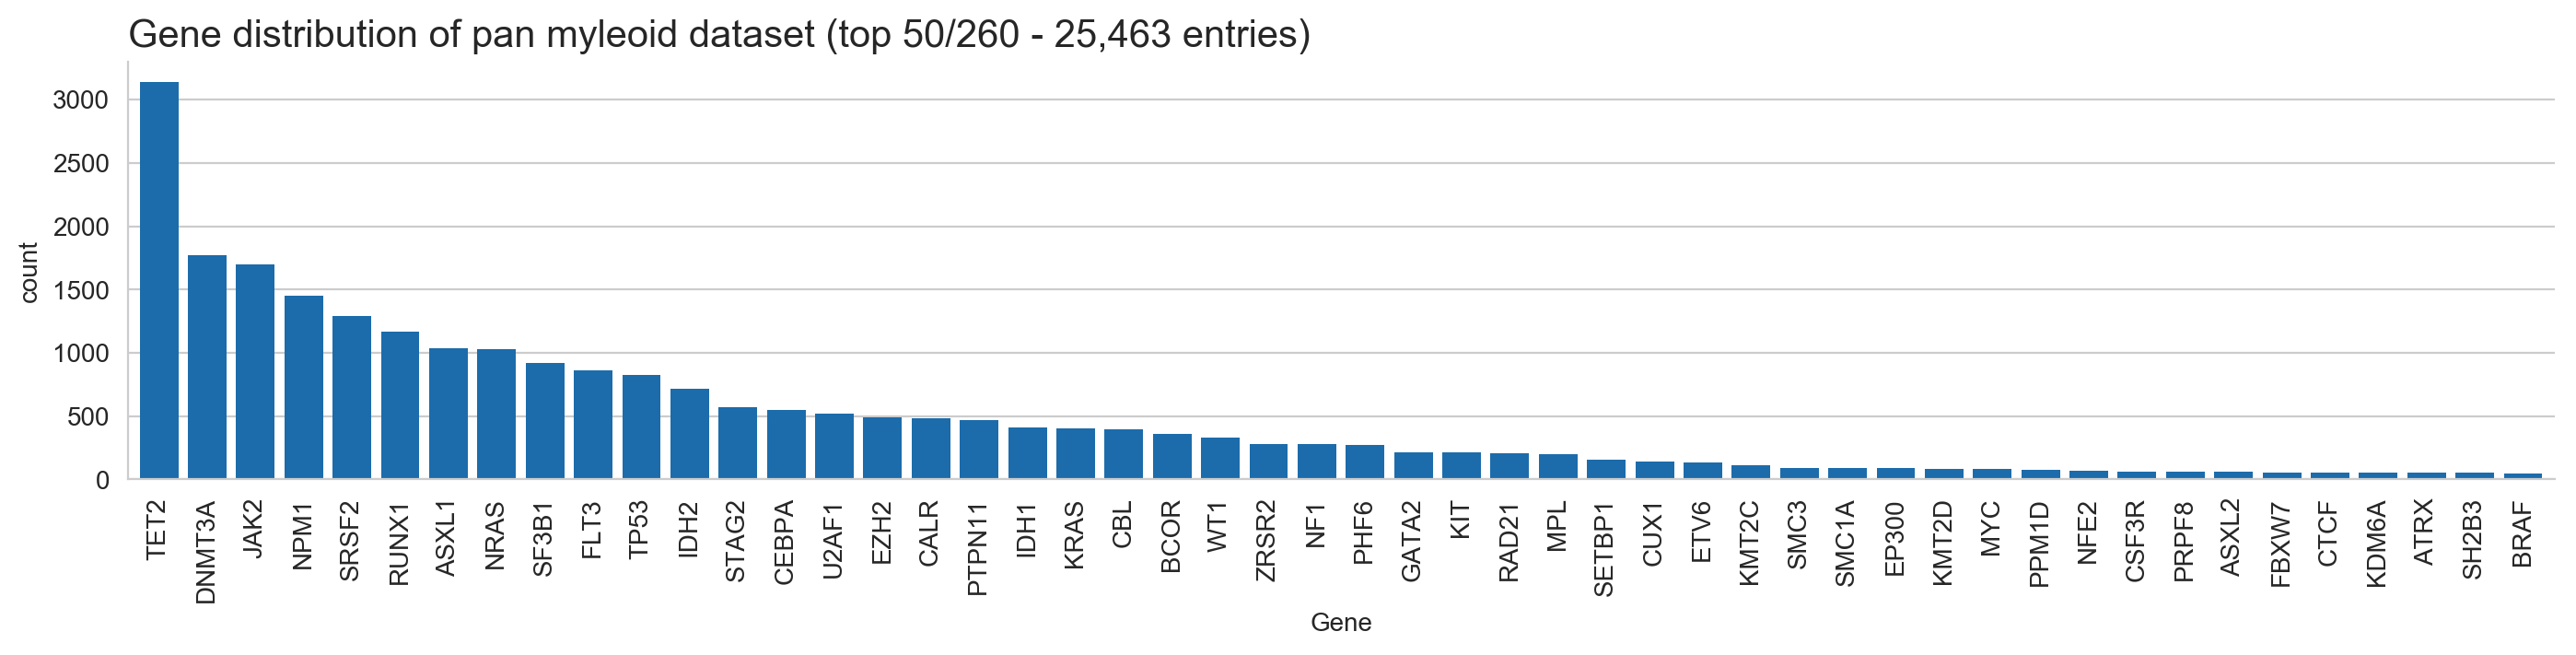
\includegraphics[scale=0.52]{{figures/fig1.png}}}

% ## Methodology
\subsection{Methodology}
\begin{itemize}
	\item Filter the indels between reported and unreported following the selected exons list. An indel is considered as reported if its beginning or end is within one of the exons of the selected exons list.
	\item Filter the substitutions between reported and unreported following the selected hotspots list. A substitution is considered as reported if it hits one of the three nucleotides of an amino acid present in the selected hotspots list.
\end{itemize}




% ########################################
% ## Unreported indels ###################
% ########################################
\newpage
\section{Unreported indels}

% ## Genes not included in the selected exons list
\subsection{Genes not included in the selected exons list}
\fbox{$\approx 31\%$} of the indels are not in the selected exons gene panel. The following plot shows the distribution of the main unreported genes:\csp
\centerline{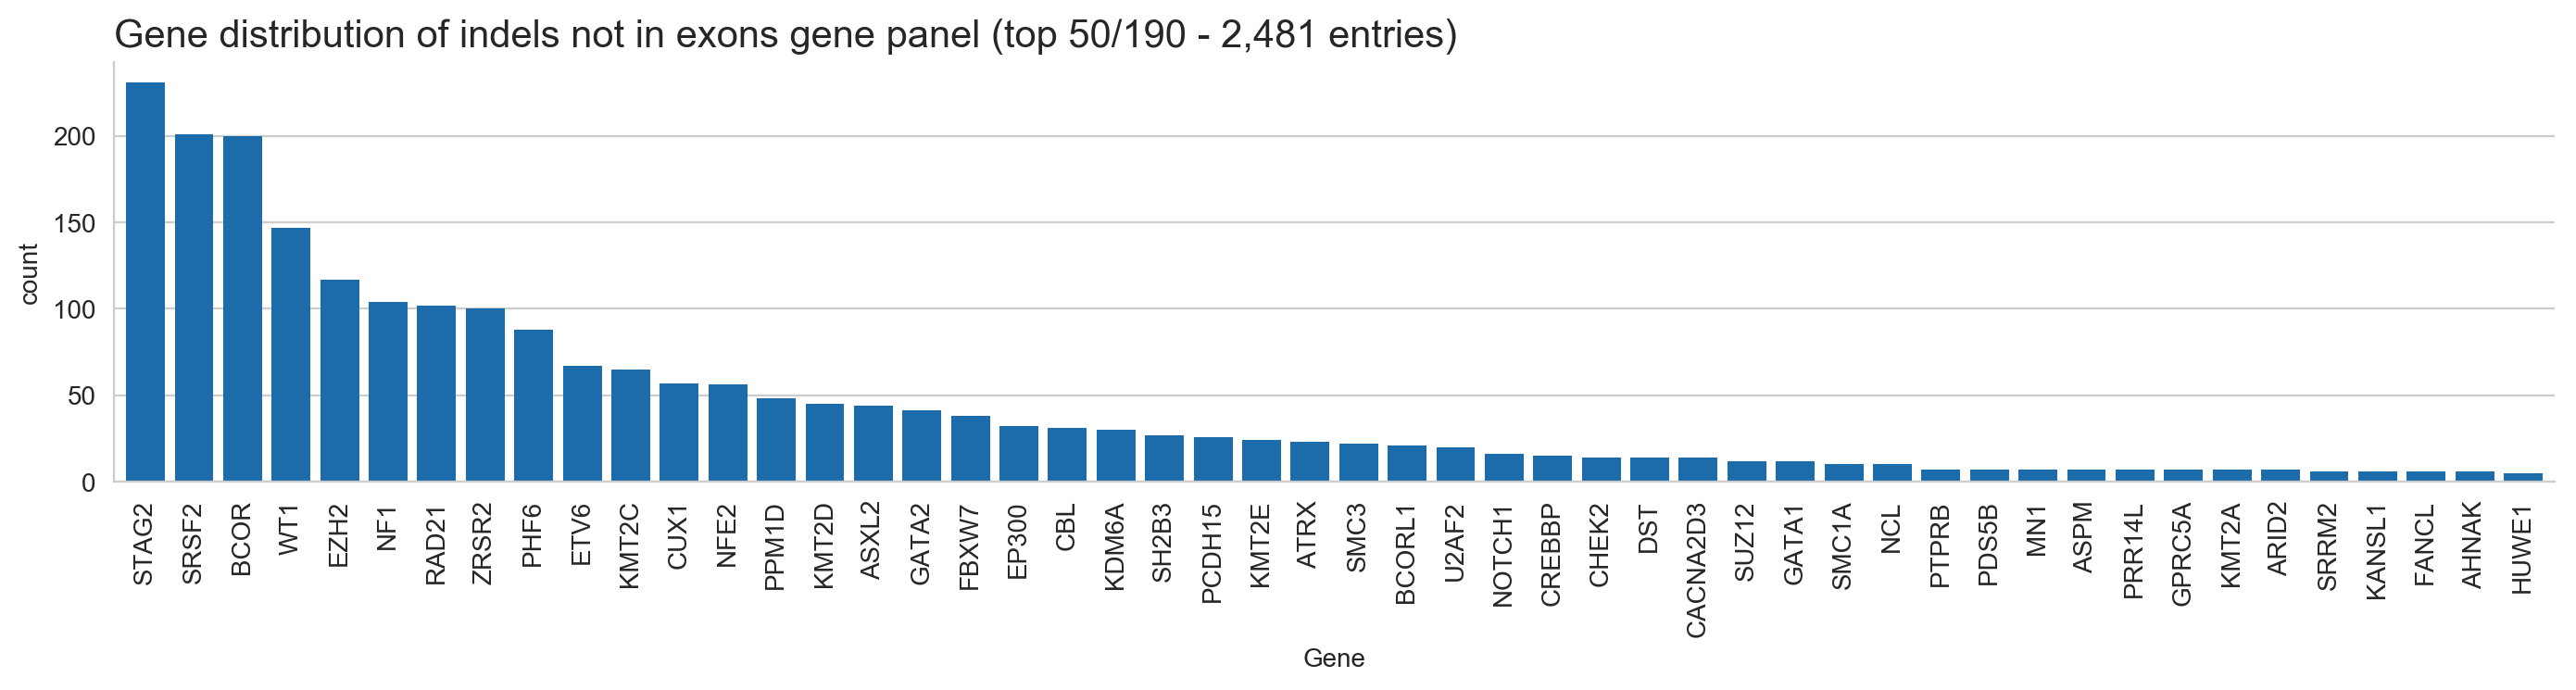
\includegraphics[scale=0.52]{{figures/fig2.png}}}

% ## Indels identified in genes with partial exon reporting
\subsection{Indels identified in genes with partial exon reporting}
Only \fbox{$\approx 2\%$} of the indels are in the selected exons gene panel, but not in the selected exons list. The following plot shows the distribution of the genes having some unreported exons:\csp
\centerline{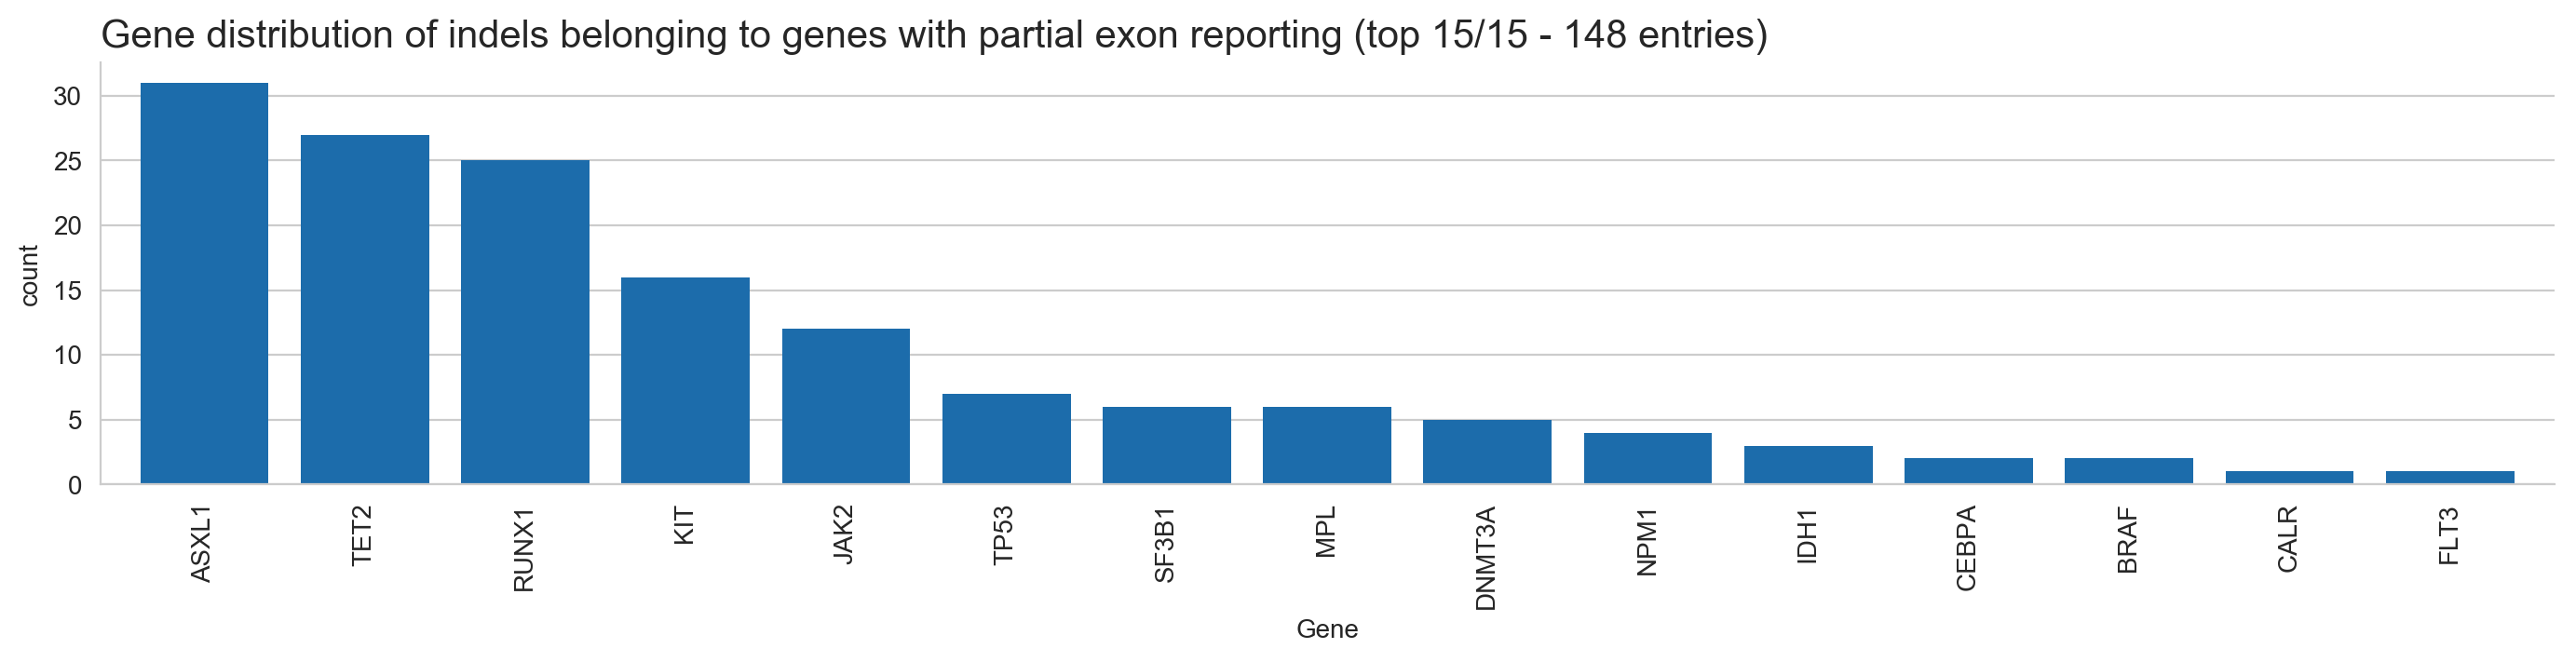
\includegraphics[scale=0.52]{{figures/fig3.png}}}

\noindent
Here is a table of the unreported exons for the genes above (NA $\Leftrightarrow$ no corresponding exon found in transcript list):\csp
{
	\small
	\begin{tabular}{|l|l|l|l|}
	    \hline
	    \textbf{gene} & \textbf{missed exons} \\ \hline
	    ASXL1   & 11 (n = 30), NA (n = 1) \\ \hline
	    TET2    & NA (n = 27) \\ \hline
	    RUNX1   & NA (n = 25) \\ \hline
	    KIT     & 8 (n = 8), 2 (n = 2), 9 (n = 1), 10 (n = 1), 5 (n = 1), 11 (n = 1), 21 (n = 1), NA (n = 1) \\ \hline
	    JAK2    & 12 (n = 5), 11 (n = 5), 19 (n = 1), NA (n = 1) \\ \hline
	    TP53    & NA (n = 7) \\ \hline
	    SF3B1   & 16 (n = 5), NA (n = 1) \\ \hline
	    MPL     & 12 (n = 3), 3 (n = 1), 11 (n = 1), NA (n = 1) \\ \hline
	    DNMT3A  & NA (n = 5) \\ \hline
	    NPM1    & 10 (n = 2), NA (n = 2) \\ \hline
	    IDH1    & 6 (n = 1), 3 (n = 1), NA (n = 1) \\ \hline
	    CEBPA   & NA (n = 2) \\ \hline
	    BRAF    & 14 (n = 1), 3 (n = 1) \\ \hline
	    CALR    & 7 (n = 1)\\ \hline
	    FLT3    & 3 (n = 1) \\ \hline
	\end{tabular}
}

% ## Summary table
\subsection{Summary table}
\begin{tabular}{|l|c|c|}
	\hline
	\textbf{indel status} & \textbf{count} & \textbf{frequency} \\ \hline
	in exons list                             & $5,267$ & $66,70\%$ \\ \hline
	not in exons gene panel                   & $2,481$ & $31,42\%$ \\ \hline
	in exons gene panel but not in exons list & $148$   & $1,87\%$  \\ \hline
\end{tabular}




% ########################################
% ## Unreported substitutions ############
% ########################################
\newpage
\section{Unreported substitutions}

% ## Genes not included in the selected hotspots list
\subsection{Genes not included in the selected hotspots list}
\fbox{$\approx 7\%$} of the substitutions are not in the selected hotspots gene panel. The following plot shows the distribution of the main unreported genes:\csp
\centerline{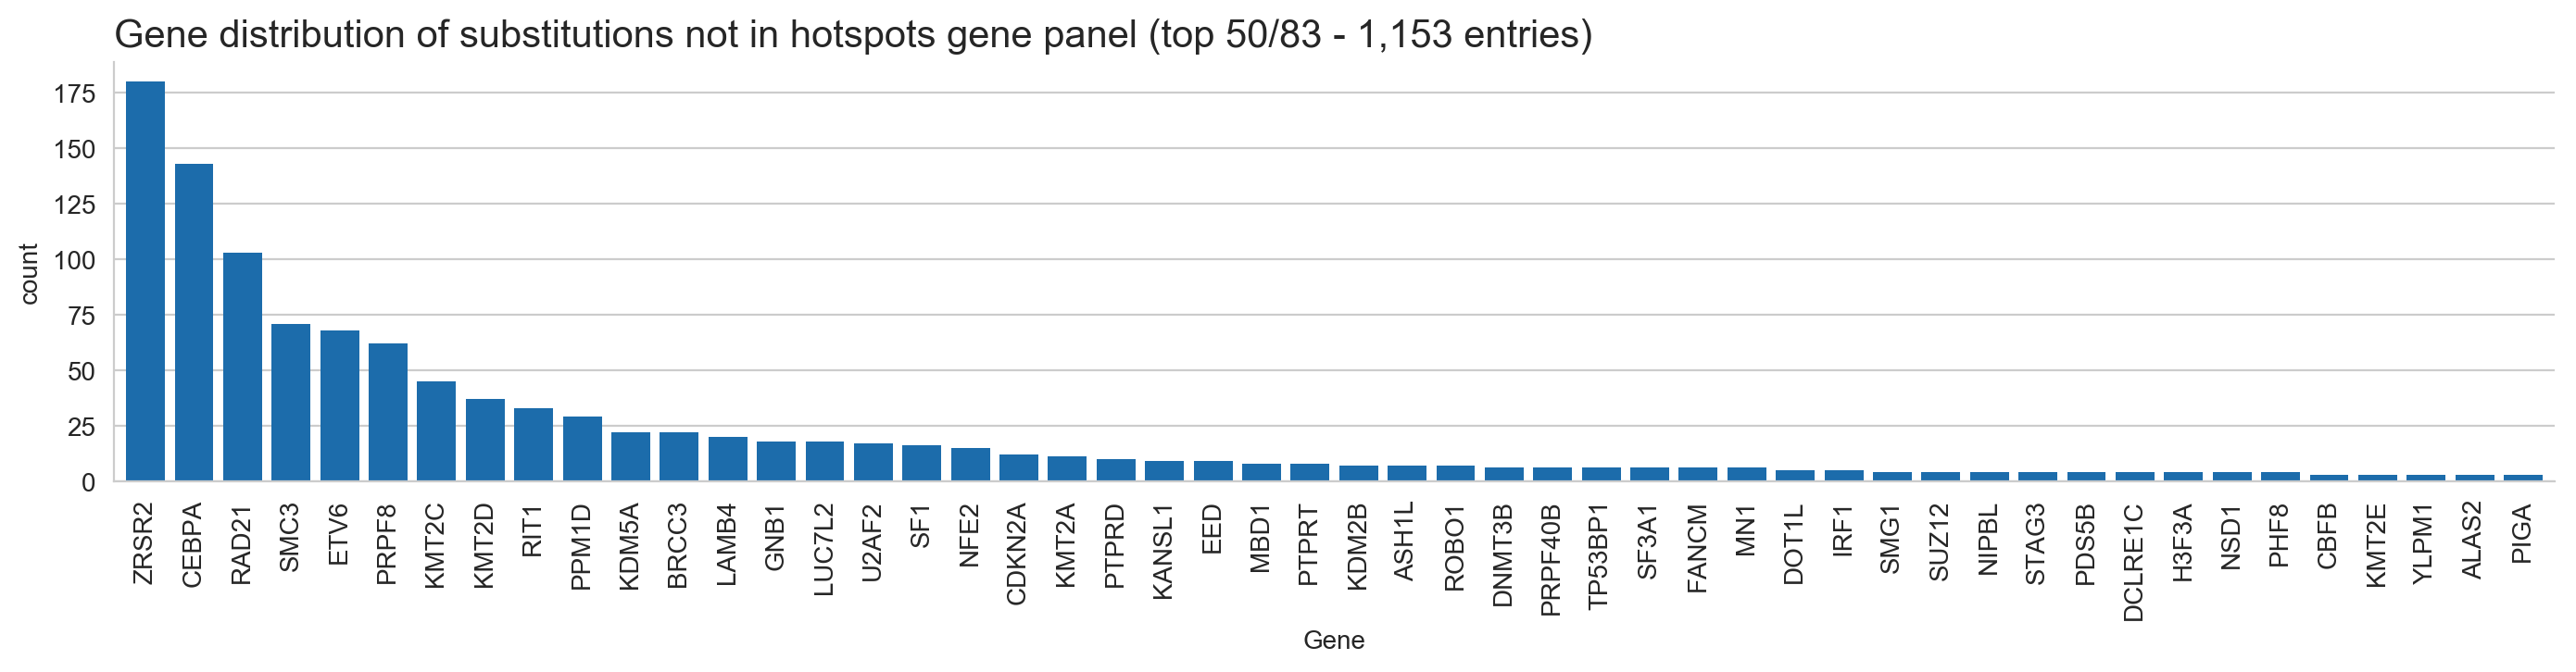
\includegraphics[scale=0.52]{{figures/fig4.png}}}

\noindent
Here is the same plot stratified by mutation consequence:\csp
\centerline{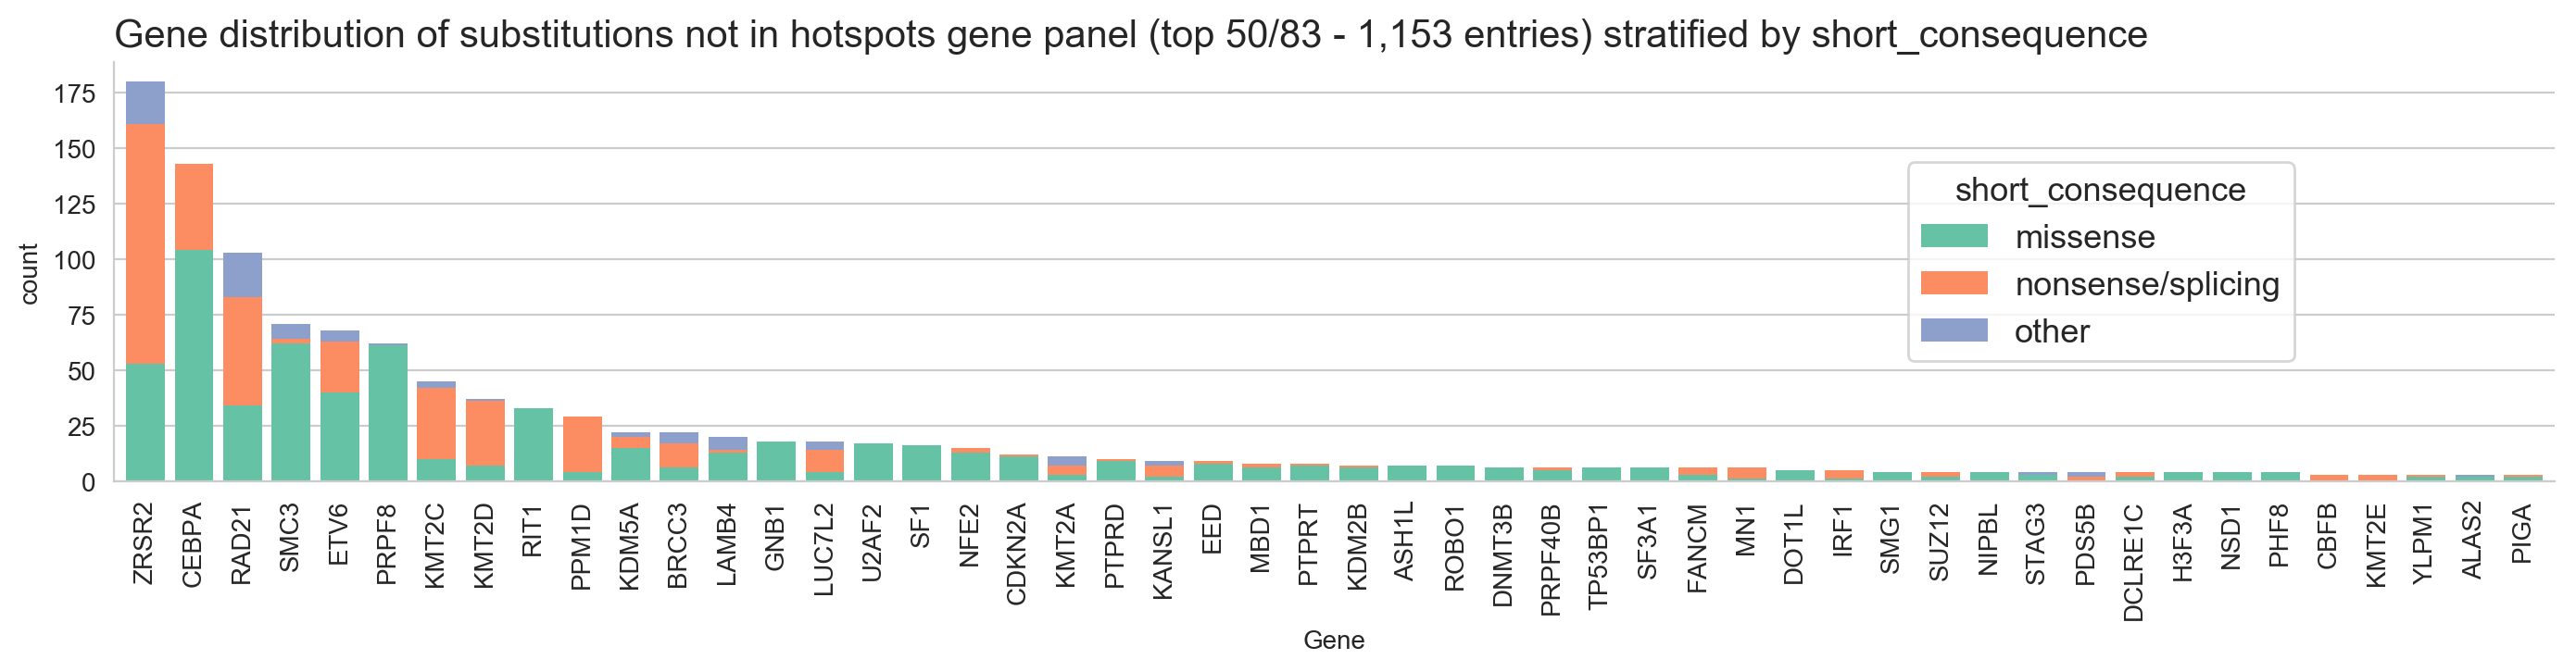
\includegraphics[scale=0.52]{{figures/fig4.2.png}}}

\noindent
Here is a figure of the 50 most recurrent unreported substitutions which are not in the selected hotspots gene panel:\csp
\centerline{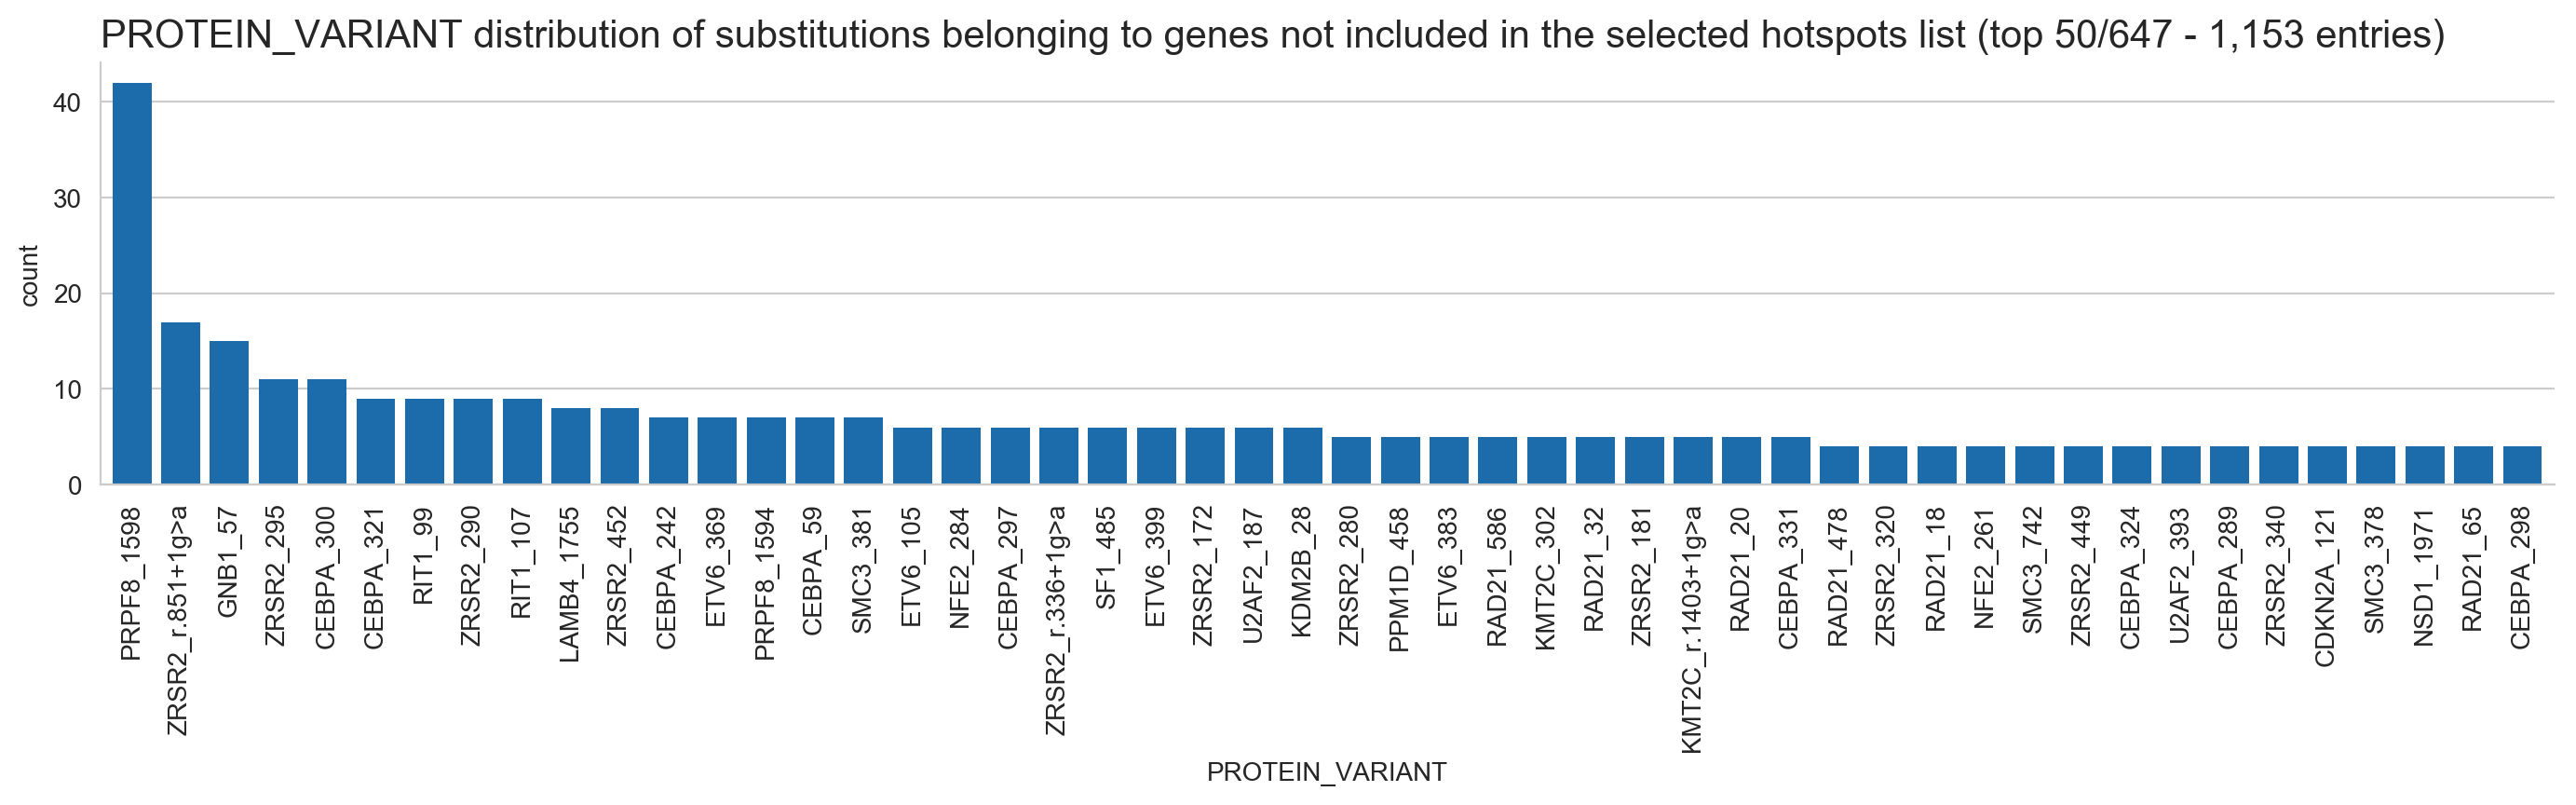
\includegraphics[scale=0.52]{{figures/fig4.3.png}}}

% ## Substitutions identified in genes with partial hotspot reporting
\subsection{Substitutions identified in genes with partial hotspot reporting}
\fbox{$\approx 31\%$} of the substitutions are in the selected hotspots gene panel, but not in the selected hotspots list. The following plot shows the distribution of the main genes having some unreported substitutions:\csp
\centerline{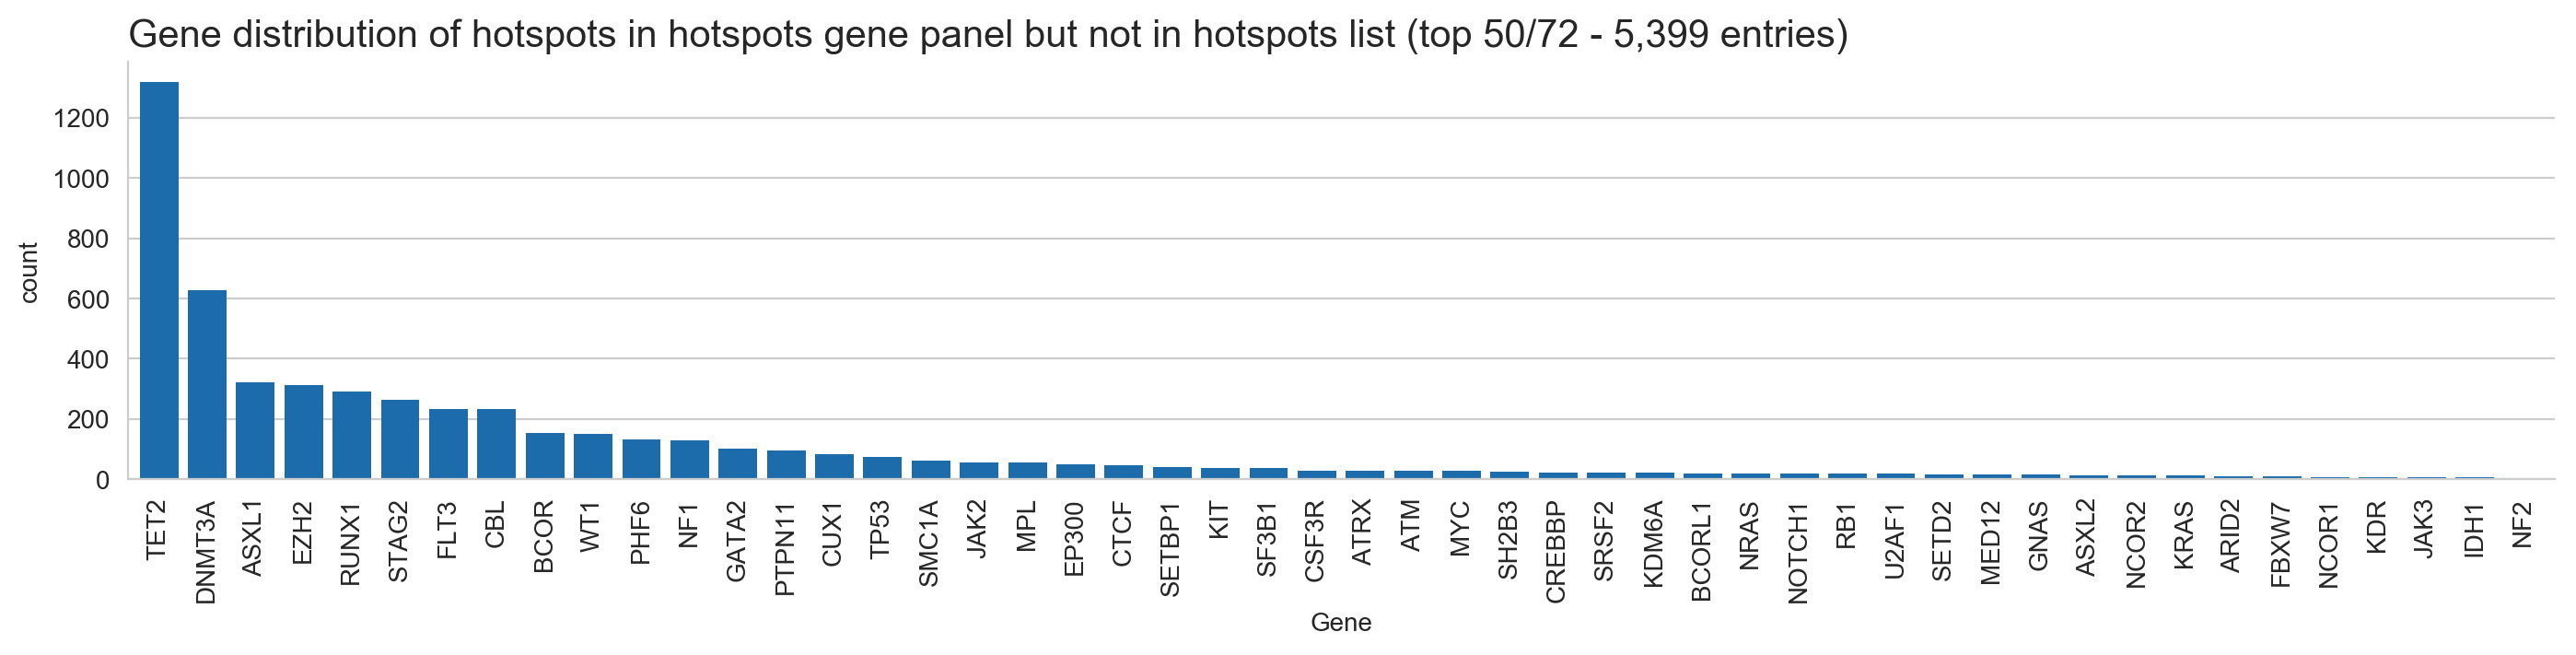
\includegraphics[scale=0.52]{{figures/fig5.png}}}

\noindent
Here is the same plot stratified by mutation consequence:\csp
\centerline{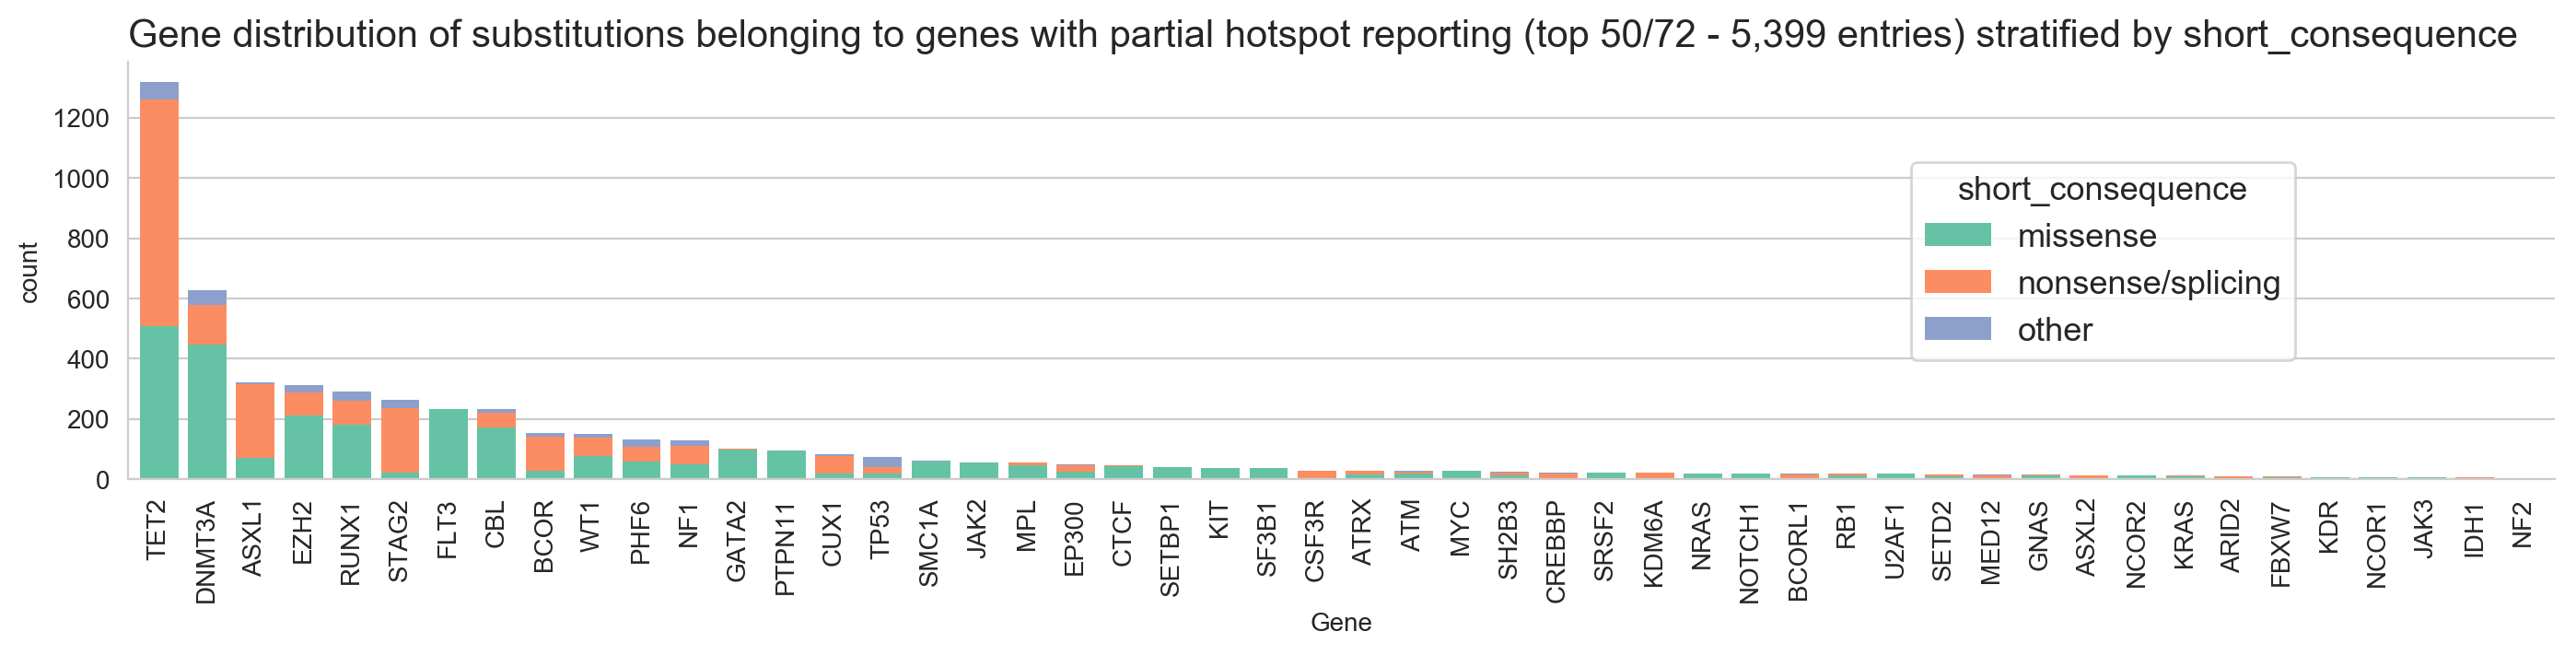
\includegraphics[scale=0.52]{{figures/fig5.2.png}}}

\noindent
Here is a figure of the 50 most recurrent unreported substitutions\footnote{\ see supplementary material 1 for the complete table}:\csp
\centerline{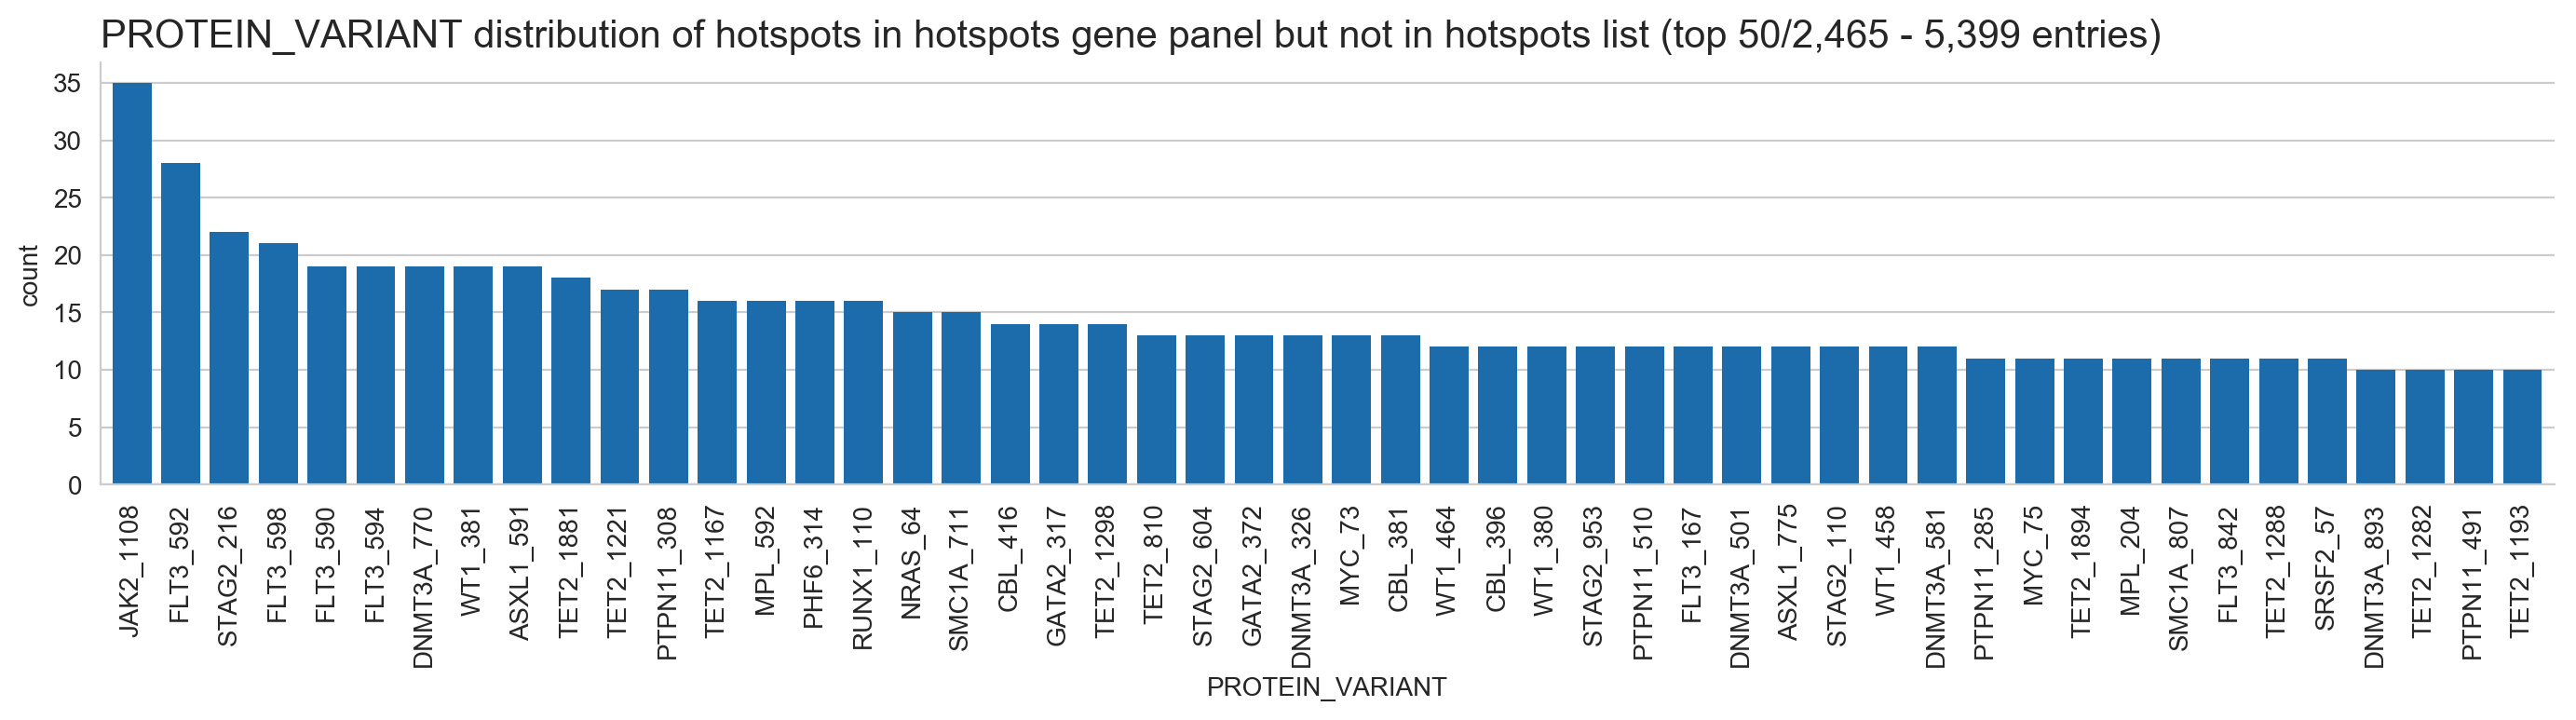
\includegraphics[scale=0.52]{{figures/fig5.3.png}}}

% ## Summary table
\subsection{Summary table}
\begin{tabular}{|l|c|c|}
	\hline
	\textbf{substitution status} & \textbf{count} & \textbf{frequency} \\ \hline
	in hotspots list                                & $11,015$ & $62,70\%$ \\ \hline
	not in hotspots gene panel                      & $1,153$  & $6,56\%$  \\ \hline
	in hotspots gene panel but not in hotspots list & $5,399$  & $30,73\%$ \\ \hline
\end{tabular}




% ########################################
% ## Summary by patient ##################
% ########################################
\newpage
\section{Summary by patient}
At the patient level, we have:
\begin{itemize}
	\item a mean of \fbox{$31\%$} oncogenic mutations unreported by patient
	\item for \fbox{$8\%$} ($711/8,966$) of the patients, \textbf{not a single oncogenic mutation reported}
\end{itemize}




% ########################################
% ## Summary by gene #####################
% ########################################
\newpage
\section{Summary by gene}
% ## Overview
\subsection{Overview}
The following plot shows the proportion of unreported mutation for the most recurrent mutated genes\footnote{\ see supplementary material 2 for the complete table}:\csp
\centerline{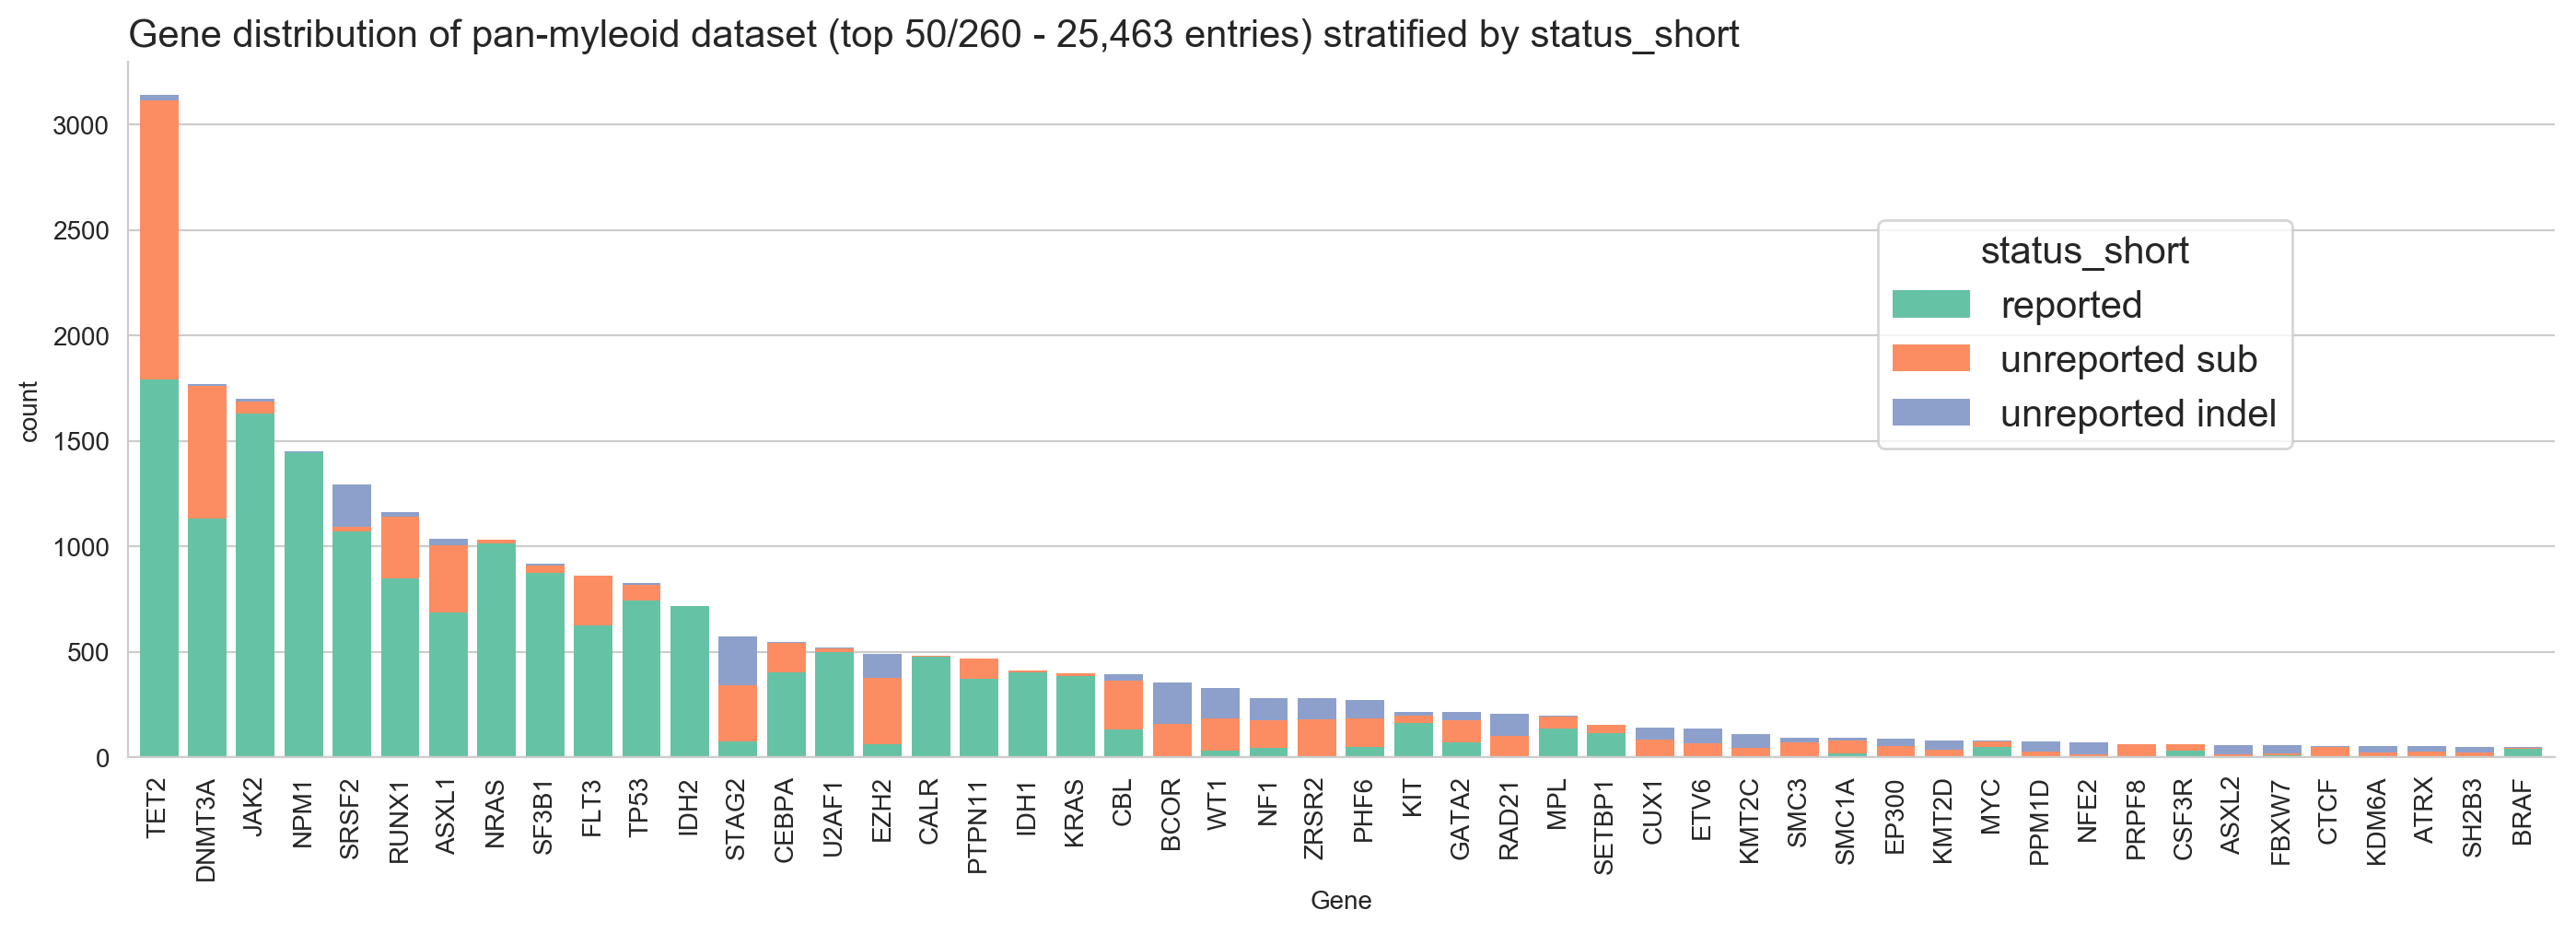
\includegraphics[scale=0.52]{{figures/fig6.png}}}\\

\noindent
In the next part we propose an analysis gene by gene for the 33 most recurrent mutated genes (see lookup table under) gathering:

%TODO clean
\begin{itemize}
	\item The OS (overall survival) plot between:
		  \begin{itemize}
			  \item \textbf{wildtype}: patients without any mutation in the studied gene
			  \item \textbf{gene name - reported}: patients with at least one reported mutation in the studied gene
			  \item \textbf{gene name - unreported}: patients with mutations in the studied gene but not a single reported mutation
		  \end{itemize}
		  Warning, the number indicated in each category represents the number of patient used to plot the curve (modulo the missing values).
	\item A pivot table showing the count of mutation reported (\checkmark) and unreported ($\times$) stratified by disease (AML, MDS or MPN) and mutation consequence (inframe, missense, nonsense/splicing, truncating or other).
	\item 4 lolliplots of the gene, two for indels (reported vs unreported) and two for substitutions (reported vs unreported).
		Warning, these lolliplots don't take into account the splicing mutations. The color of the mutation circle represents its consequence, the size of the mutation circle represents its occurence in the dataset, see legend:\\\\
		\includegraphics[width=17cm]{{lolliplots_legend.png}}\\
\end{itemize}

\noindent
Lookup table gene $\leftrightarrow$ page: \\\\
\begin{tabular}{lr|lr|lr|lr|lr|lr}
\toprule
gene & page & gene & page & gene & page & gene & page & gene & page & gene & page \\
\midrule
    TET2   & 7  & ASXL1  & 13 & STAG2  & 19 & IDH1   & 25 & ZRSR2  & 31 & SETBP1 & 37 \\
    DNMT3A & 8  & NRAS   & 14 & CEBPA  & 20 & KRAS   & 26 & PHF6   & 32 & CUX1   & 38 \\
    JAK2   & 9  & SF3B1  & 15 & U2AF1  & 21 & CBL    & 27 & KIT    & 33 & ETV6   & 39 \\
    NPM1   & 10 & FLT3   & 16 & EZH2   & 22 & BCOR   & 28 & GATA2  & 34 \\
    SRSF2  & 11 & TP53   & 17 & CALR   & 23 & WT1    & 29 & RAD21  & 35 \\
    RUNX1  & 12 & IDH2   & 18 & PTPN11 & 24 & NF1    & 30 & MPL    & 36 \\
\bottomrule
\end{tabular}

% ## By gene summary

\definecolor{c_purple}{RGB}{137,110,142}
\definecolor{c_orange}{RGB}{238,134,124}

\setlength{\fboxrule}{1pt}
\foreach \gene in {TET2, DNMT3A, JAK2, NPM1, SRSF2, RUNX1, ASXL1, NRAS, SF3B1, FLT3, TP53, IDH2, STAG2, CEBPA, U2AF1, EZH2, CALR, PTPN11, IDH1, KRAS, CBL, BCOR, WT1, NF1, ZRSR2, PHF6, KIT, GATA2, RAD21, MPL, SETBP1, CUX1, ETV6}
{
	\newpage
	\subsection{\gene}
	
	\begin{multicols}{2}
		% OS plot
		\noindent
		\includegraphics[width=8.5cm, height=8.5cm]{{OS_plots/OS_\gene.png}}
		
		\columnbreak
		% pivot table with small fontsize
		{
			\setlength\tabcolsep{4pt} % change col separation length
			\centerline{\input{dataframes/gene_summary/\gene_summary.txt}}
		}
	\end{multicols}
	
	% 4 lolliplots
	
	\subsubsection*{Indels}
	% reported indels
	\noindent
	\textcolor{c_purple}{\textbf{reported}}\csp
	\IfFileExists{lolliplots/indels/\gene_reported.png}
	{
		\fcolorbox{c_purple}{white}{\centerline{\includegraphics[scale=0.1]{{lolliplots/indels/\gene_reported.png}}}}\\
	}
	{ This gene was not reported for exons (or no reported mutation was found in the dataset).\\ }
	
	% unreported indels
	\noindent
	\textcolor{c_orange}{\textbf{unreported}}\csp
	\IfFileExists{lolliplots/indels/\gene_unreported.png}
	{
		% TET2, DNMT3A and RUNX1 unreported indels have been checked and are just one base pair from the beginning/end of the exons, they would have been reported
		\ifthenelse{\equal{\gene}{TET2} \OR \equal{\gene}{DNMT3A} \OR \equal{\gene}{RUNX1}}
		{ No unreported indel found.\\ } 
		{ \fcolorbox{c_orange}{white}{\centerline{\includegraphics[scale=0.1]{{lolliplots/indels/\gene_unreported.png}}}} }
	}
	{ No unreported indel found.\\ }
		
	\subsubsection*{Substitutions}
	% reported substitutions
	\noindent
	\textcolor{c_purple}{\textbf{reported}}\csp
	\IfFileExists{lolliplots/substitutions/\gene_reported.png}
	{
		\fcolorbox{c_purple}{white}{\centerline{\includegraphics[scale=0.1]{{lolliplots/substitutions/\gene_reported.png}}}}\\
	}
	{ This gene was not reported for hostpots (or no reported mutation was found in the dataset).\\ }
	
	% unreported substitutions
	\noindent
	\textcolor{c_orange}{\textbf{unreported}}\csp
	\IfFileExists{lolliplots/substitutions/\gene_unreported.png}
	{
		\fcolorbox{c_orange}{white}{\centerline{\includegraphics[scale=0.1]{{lolliplots/substitutions/\gene_unreported.png}}}}
	}
	{ No unreported substitution found.\\ }
	
	% TET2 special note
	\ifthenelse{\equal{\gene}{TET2}} {\textsuperscript{*} likely germline infiltration}{}
}




% ########################################
% ## Supplementary material ##############
% ########################################
\newpage
\section{Supplementary material}

% ## Unreported substitutions table (with count $\geq 5$)
\subsection{Unreported substitutions table (with count $\geq 5$)}
Table of the substitutions identified in genes with partial hotspot reporting.
\begin{center}
	\input{dataframes/unreported_substitutions_table.txt}
\end{center}

% ## Gene summary table
\newpage
\subsection{Gene summary table}
\begin{center}
	\setlength\tabcolsep{3pt} % change col separation length
	\input{dataframes/gene_summary_table.txt}
\end{center}




\end{document}
